\vspace{-0.5em}
\section{Introduction}
An increasingly popular approach for fast query processing on large datasets is to pre-compute query results.
These pre-computed query results, known as Materialized views (MVs), have been well studied over the last 30 years in the
research community \cite{LarsonY85, gupta1995maintenance, chirkova2011materialized}.
MVs are now supported by all major commercial vendors and many key ideas from MV research have been applied in linear algebra and machine learning \cite{nikolic2014linview, zhang2014mat}.

However, as with any pre-computation, when the base data is updated MVs can become \emph{stale}. 
There has been substantial work in deriving incremental updates (incremental maintenance) for many classes of MVs and optimizing their execution \cite{chirkova2011materialized, DBLP:journals/vldb/KochAKNNLS14}.
In emerging MV applications, such as real time analytics \cite{rainbird}, views are growing in size and base data updates are happening at an ever increasing rate.
For frequently changing tables, eager incremental maintenance can be inefficient since every update to the base data requires updating all the dependent views; a challenge that only becomes worse in a distributed environment.
Even with recently proposed optimizations such as DBToaster by Kock et al. \cite{DBLP:journals/vldb/KochAKNNLS14}, these bottlenecks can force the deferal of view
maintenance \cite{chirkova2011materialized, zhou2007lazy, DBLP:conf/sigmod/ColbyGLMT96}.
As a result, in production environments, it is common to batch updates together to amortize overheads.
Batch sizes are set according to system constraints and in production systems can vary from a few seconds to even nightly.  

While increasing the batching period gives the user more flexibility in scheduling around system constraints, a disadvantage is that MVs become increasingly stale between maintenance periods.
As a result, queries using those MVs can return incorrect answers in the interim.
Other than an educated guess based on trends in prior data, in general, the user has no way of knowing how close or how far they are from the true answer.
Thus, any amount of staleness is potentially dangerous, and this presents us a dichotomy between facing the cost of maintenance or coping with consequences of inaccuracy.
In this paper, we explore an intruiging middle ground, namely, for aggregate queries, we can derive a bounded approximation for the correct answer for a fraction of the maintenance cost. 

%This observation leads us to the main insight behind our work; namely, that a data cleaning approach can be applied to mitigate the negative impacts of deferred MV maintenance.

\begin{figure}[t] \vspace{-2em}
\centering
 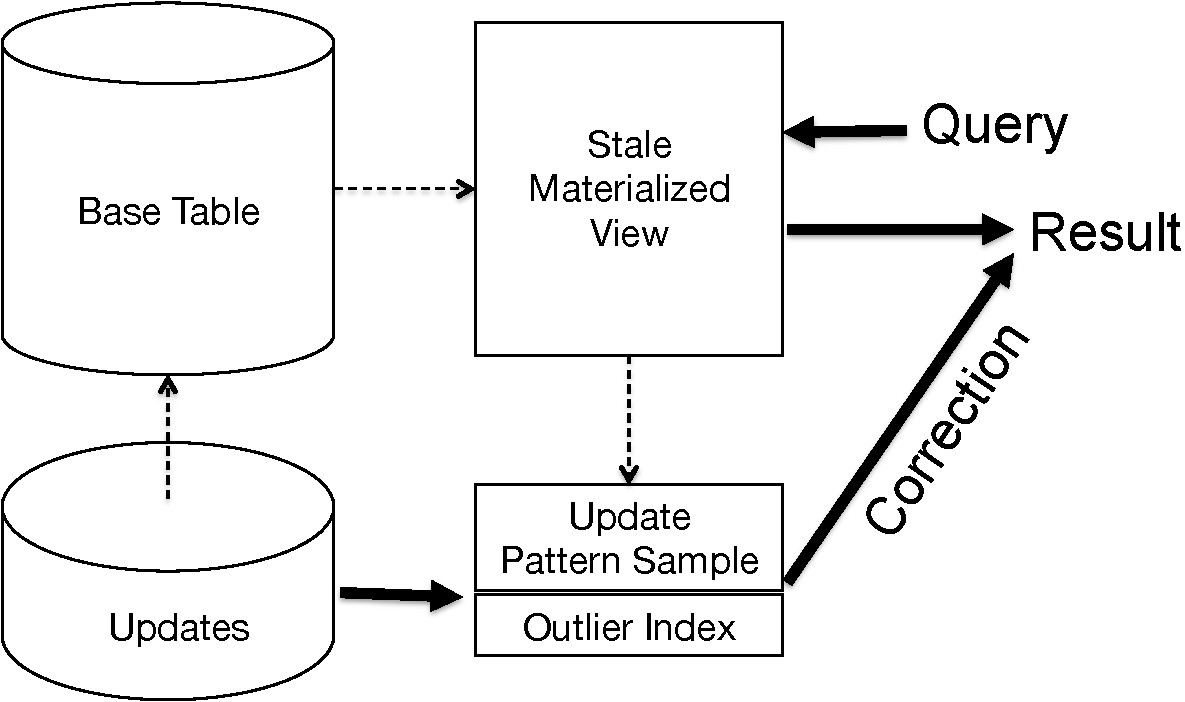
\includegraphics[scale=0.27]{figs/sys-arch.pdf} \vspace{-.25em}
 \caption{Deferred maintenance can lead to stale MVs which have incorrect, missing, and superfluous rows. In \svc, we pose this as a data cleaning problem and show that we can use a sample of clean (up-to-date) rows from an MV to correct inaccurate query results on stale views. \label{sys-arch}}\vspace{-1.75em}
\end{figure}

Our method relies on modeling queries on stale MVs as a data cleaning problem.
As with dirty data, a staleness results in incorrect, missing, or superfluous rows.
Data cleaning has been studied extensively in the literature (e.g., see Rahm and Do for a survey\cite{rahm2000data}) but increasing data volumes have led to development of new, efficient sampling-based approaches for coping with dirty data.   
In our prior work, we developed the SampleClean framework for scalable aggregate query processing on dirty data \cite{wang1999sample}.
Since data cleaning is often expensive, we proposed cleaning a sample of data using this sample to improve the results of aggregate queries on the full dataset.
Since stale MVs are dirty data, an approach similar to SampleClean raises a new possibility of using a sample of ``clean'' rows in the MV to return more accurate query results.

\svcfull (\svc illustrated in Figure~\ref{sys-arch}) provides a framework that efficiently answers aggregate queries on a stale MV.
Using the view definition, it derives an efficient relational expression that materializes a uniform sample of ``clean" (up-to-date) rows.
We use the clean sample of rows to estimate a result for an aggregate query on the view.
The estimates from this procedure, while approximate, are up-to-date in the sense that they reflect the most recent data. 
The approximation error due to sampling is more manageable than staleness because: (1) the uniformity of sampling allows us to apply theory from statistics such as the Central Limit Theorem to give tight bounds on approximate results, and (2) the approximate error is parametrized by the sample size which the user can control trading off accuracy for computation.
\svc is complementary to existing deferred maintenance approaches.
When the MVs become stale between maintenance cycles, we apply \svc for a far smaller cost than having to maintain the entire view but still get approximate, up-to-date answers.

%Both MVs and queries can be complex.

To summarize, our contributions are as follows: (1) we formalize maintenance of a sample MV as a data cleaning operation on the sample, (2) we propose an optimization technique that materializes the clean sample efficiently while preserving correctness, (3) we derive a query processing approach to answer aggregate queries accurately using the clean sample, (4) we propose an outlier index to reduce sensitivity to skewed datasets, and (5) we evaluate our approach on real and synthetic datasets confirming that indeed sampling can reduce view maintenance time while providing accurate query results. 
%\end{itemize}

The paper is organized as follows: 
In Section~\ref{sec-background}, we give the necessary background for our work.
Next, in Section~\ref{sec-arch}, we formalize the problem.
In Sections~\ref{sampling} and~\ref{correction}, we describe the sampling and query processing of our technique.
In Section~\ref{outlier}, we describe the outlier indexing framework.
Then, in Section~\ref{exp}, we evaluate our approach.
Finally, we discuss Related Work in Section~\ref{related}.
In Section~\ref{sec:disc}, we discuss the limitations and future opportunities of our approach, and we present our Conclusions in Section~\ref{conclusion}.
%Full versions of our proofs and experimental details are available in our extended technical report \cite{technicalReport}.
